\documentclass[10pt,a4paper]{amsart}
\usepackage[margin=19mm]{geometry}
\usepackage{amsmath,amssymb,mathtools}
\usepackage[scr=rsfs,cal=euler]{mathalfa}
\usepackage{xfrac}
\usepackage[unicode,hidelinks,bookmarks=false]{hyperref}
\newcommand{\ie}{i.e.\ }
\newcommand{\cf}{cf.\ }
\newcommand{\resp}{respectively\ }
\newcommand{\Subsection}{\subsection}
\providecommand{\nobreakdash}{\nobreak\hbox{-}}
\setlength{\emergencystretch}{2em}
\multlinegap0pt
\usepackage{mathtools}
\usepackage{enumitem}
\usepackage{booktabs}
\usepackage{float}
\usepackage{tikz}
\usepackage{xurl}
\newtheorem{theorem}{Theorem}[section]
\newtheorem{corollary}[theorem]{Corollary}
\newtheorem{lemma}[theorem]{Lemma}
\newtheorem{proposition}[theorem]{Proposition}
\newtheorem{definition}[theorem]{Definition}
\newtheorem{example}[theorem]{Example}
\newtheorem{question}[theorem]{Question}
\newtheorem{remark}[theorem]{Remark}
\numberwithin{equation}{section}
\newcommand{\NN}{\mathcal N}
\newcommand{\DD}{\mathcal D}
\newcommand{\Ho}{\mathcal H_{\!o}}
\newcommand{\Cl}{\operatorname{Cl}}
\newcommand{\CN}{\operatorname{CN}}
\newcommand{\pd}{\operatorname{pdim}}
\newcommand{\depth}{\operatorname{depth}}
\newcommand{\reg}{\operatorname{reg}}
\newcommand{\mult}{\operatorname{e}}
\begin{document}
\title[A Complete Classification of 2-Linear Neighborhood Complexes]{A Complete Classification of 2-Linear Neighborhood Complexes}
\author{Mohammed Rafiq Namiq}
\date{}
\maketitle
\noindent\emph{Source and licence.} A Complete Classification of 2-Linear Neighborhood Complexes. Version arXiv:2606.03573v2 (CC BY 4.0). This material is distributed under the Creative Commons Attribution 4.0 International licence, http://creativecommons.org/licenses/by/4.0/, as recorded in the arXiv OAI licence metadata for this exact version and shown on the abstract page https://arxiv.org/abs/2606.03573v2. Full rights notice: licenses/arxiv-2606.03573-CC-BY-4.0.txt.\par\smallskip
\noindent\textit{Editorial scope.} Counted unit: the original \texttt{theorem} environment \texttt{thm:all-betti} at source lines 892--921 together with its complete proof at lines 923--962; the delivered document keeps source lines 249--963 so that every referenced label and every citation resolves inside it. Native editable source is the paper's own concatenated TeX; the AMS wrapper is editorial formatting only. No publisher class, upstream script or unrelated artwork is redistributed.
	\begin{lemma}\label{lem:helly-flag}
		For a nonempty finite simple graph \(G\), the following are equivalent:
		\begin{enumerate}[label=\textup{(\roman*)}]
			\item the open neighborhoods of \(G\) form a Helly family;
			\item every nonempty clique \(Q\) of \(\CN(G)\) is contained in
			\(N_G(w)\) for some \(w\in V\);
			\item \(\NN(G)=\Cl(\CN(G))\);
			\item \(\NN(G)\) is flag on the ground set \(V\).
		\end{enumerate}
	\end{lemma}
	
	\begin{proof}
		Let \(Q\subseteq V\) be nonempty. The indexed family
		\((N_G(q))_{q\in Q}\) is pairwise intersecting exactly when every two
		vertices of \(Q\) have a common neighbor, or equivalently, when \(Q\) is a
		clique of \(\CN(G)\). Moreover,
		\[
		\bigcap_{q\in Q}N_G(q)\ne\varnothing
		\quad\Longleftrightarrow\quad
		Q\subseteq N_G(w)\text{ for some }w\in V.
		\]
		Thus \textup{(i)} and \textup{(ii)} are equivalent.
		
		Every face of \(\NN(G)\) is contained in an open neighborhood. Any two
		vertices of such a face therefore have a common neighbor, and hence
		\[
		\NN(G)\subseteq\Cl(\CN(G)).
		\]
		Condition \textup{(ii)} gives the reverse inclusion, proving the equivalence
		of \textup{(ii)} and \textup{(iii)}.
		
		Finally, the edges of \(\CN(G)\) are precisely the faces of \(\NN(G)\)
		with two vertices. Therefore \(\NN(G)\) is flag on the prescribed ground set
		\(V\) if and only if it equals \(\Cl(\CN(G))\). This formulation also covers
		isolated vertices. If \(v\) is isolated in \(G\), then \(\{v\}\) is a
		clique of \(\CN(G)\) but not a face of \(\NN(G)\); consequently, both
		\textup{(iii)} and \textup{(iv)} fail.
	\end{proof}
	
	A hypergraph on \(V\) is a \emph{hypertree} if every hyperedge is nonempty and
	there exists a tree on \(V\) in which each hyperedge induces a subtree. We
	treat repeated open neighborhoods as indexed hyperedges. Passing to the family
	of distinct hyperedges preserves both the Helly property and subtree
	representability. Conversely, duplicating a nonempty hyperedge adds a true twin
	to the line graph and therefore preserves chordality. The classical hypertree
	criterion consequently applies to the indexed family without modification.
	
	\begin{proposition}\label{prop:background}
		For a nonempty finite simple graph \(G\), the following are equivalent:
		\begin{enumerate}[label=\textup{(\roman*)}]
			\item \(I_{\NN(G)}\) has a \(2\)-linear resolution;
			\item the open neighborhoods of \(G\) form a Helly family, and \(\CN(G)\) is chordal;
			\item \(\Ho(G)=(N_G(v))_{v\in V}\) is a hypertree.
		\end{enumerate}
		The conditions are independent of \(\operatorname{char}\Bbbk\), and any
		graph satisfying them has no isolated vertices.
	\end{proposition}
	
	\begin{proof}
		The ideal \(I_{\NN(G)}\) is nonzero because no open neighborhood contains the
		full vertex set. Assume first that \textup{(i)} holds. Since a \(2\)-linear
		resolution forces \(I_{\NN(G)}\) to be generated in degree \(2\), the complex
		\(\NN(G)\) is flag on \(V\). Lemma~\ref{lem:helly-flag} then shows that the open neighborhoods of \(G\)
		form a Helly family and yields the equalities
		\[
		\NN(G)=\Cl(\CN(G)),
		\qquad
		I_{\NN(G)}=I\bigl(\overline{\CN(G)}\bigr).
		\]
		Fr\"oberg's theorem \cite[Theorem~1]{Froberg1990} now implies that
		\(\CN(G)\) is chordal. Hence \textup{(i)} implies \textup{(ii)}.
		
		Conversely, assume \textup{(ii)}. Lemma~\ref{lem:helly-flag} again yields
		\[
		I_{\NN(G)}=I\bigl(\overline{\CN(G)}\bigr).
		\]
		The right side is the edge ideal of the complement of the chordal graph
		\(\CN(G)\). Fr\"oberg's theorem therefore gives a \(2\)-linear resolution,
		proving the equivalence of \textup{(i)} and \textup{(ii)}.
		
		Under the identification of \(v\) with the indexed hyperedge \(N_G(v)\), the
		line graph of \(\Ho(G)\) is \(\CN(G)\). The classical characterization of hypertrees by the Helly property
		and chordality \cite{BrandstadtDraganChepoiVoloshin1998} proves the
		equivalence of \textup{(ii)} and \textup{(iii)}. All three conditions are
		combinatorial and are therefore independent of \(\operatorname{char}\Bbbk\).
		Finally, \textup{(ii)} excludes isolated vertices: for every \(v\in V\), the
		singleton indexed family \(\{N_G(v)\}\) must have nonempty intersection.
	\end{proof}

	Our convention for the ground set makes isolated vertices algebraically visible.
	The following observation records exactly how they alter the resolution.

	\begin{proposition}\label{prop:isolated-vertices}
		Let \(Z\) be the set of isolated vertices of \(G\), let \(t=|Z|\), and put
		\(G^{\circ}=G-Z\). Assume first that \(G^{\circ}\) is nonempty. With
		\[
		S^{\circ}=\Bbbk[x_v:v\in V(G^{\circ})],
		\qquad S=S^{\circ}[x_z:z\in Z],
		\]
		one has
		\[
		I_{\NN(G)}=I_{\NN(G^{\circ})}S+(x_z:z\in Z)
		\]
		and
		\begin{equation}\label{eq:isolated-convolution}
		\beta^{S}_{i,j}\bigl(\Bbbk[\NN(G)]\bigr)
		=
		\sum_{a=0}^{\min\{t,i\}}
		\binom ta\,
		\beta^{S^{\circ}}_{i-a,j-a}
		\bigl(\Bbbk[\NN(G^{\circ})]\bigr).
		\end{equation}
		If every vertex of \(G\) is isolated, then
		\(I_{\NN(G)}=(x_v:v\in V(G))\) and
		\(\beta^S_{i,i}=\binom{|V(G)|}{i}\).
	\end{proposition}

	\begin{proof}
		No face of \(\NN(G)\) contains a vertex of \(Z\), while a subset of
		\(V(G^{\circ})\) is a face of \(\NN(G)\) exactly when it is a face of
		\(\NN(G^{\circ})\). This proves the ideal identity. Hence
		\[
		\Bbbk[\NN(G)]
		\cong
		\Bbbk[\NN(G^{\circ})]
		\otimes_{\Bbbk}
		\Bbbk[x_z:z\in Z]/(x_z:z\in Z).
		\]
		Tensoring a minimal \(S^{\circ}\)-resolution of the first factor with the
		Koszul resolution of the second factor gives a minimal \(S\)-resolution and
		yields \eqref{eq:isolated-convolution}. When all vertices are isolated, the resolution is the Koszul resolution of
		the residue field.
	\end{proof}
	
	\section{A structural reformulation in graph terms}\label{sec:structure}
	
	Proposition~\ref{prop:background} can be stated directly in terms of the
	cycles and neighborhoods of \(G\).
	
	Let \(G=(X\sqcup Y,E)\) be bipartite. Vertices in different color classes
	cannot have a common neighbor, and hence
	\begin{equation}\label{eq:half-square-decomposition}
		\CN(G)=\CN(G)[X]\sqcup\CN(G)[Y].
	\end{equation}
	The two summands are the half squares of \(G\) on \(X\) and on \(Y\)
	\cite{LeLe2019}.
	
	
	
	\begin{definition}
		Let
		\[
		C=x_1 y_1 x_2 y_2\cdots x_q y_q x_1,\qquad q\ge4,
		\]
		be an induced cycle of \(G=(X\sqcup Y,E)\), with \(x_i\in X\) and
		\(y_i\in Y\). A \emph{filling on \(X\)} of \(C\) is a common neighbor in
		\(G\) of two nonconsecutive vertices among \(x_1,\ldots,x_q\). A
		\emph{filling on \(Y\)} is defined symmetrically. The cycle is
		\emph{filled on both sides} if it has a filling on \(X\) and a filling on \(Y\).
	\end{definition}
	
	Because \(C\) is induced, every vertex that provides a filling lies outside
	\(V(C)\). A filling on \(X\) is provided by a vertex of \(Y\), whereas a
	filling on \(Y\) is provided by a vertex of \(X\). Thus the label records the
	color class of the cycle vertices that share the additional common neighbor.
	
	\begin{example}\label{ex:bifilled-cycle}
		Let $C=x_1y_1x_2y_2x_3y_3x_4y_4x_5y_5x_1$ be an induced \(10\)-cycle. If \(z_Y\in Y\) and \(z_X\in X\) satisfy
		\[
		N_G(z_Y)\cap V(C)=\{x_1,x_3,x_5\},
		\qquad
		N_G(z_X)\cap V(C)=\{y_1,y_3\},
		\]
		then \(z_Y\) provides a filling on \(X\), while \(z_X\) provides a filling on \(Y\).
		Hence \(C\) is filled on both sides. Figure~\ref{fig:bifilled-cycle} illustrates the two fillings.
		
		\begin{figure}[H]
			\centering
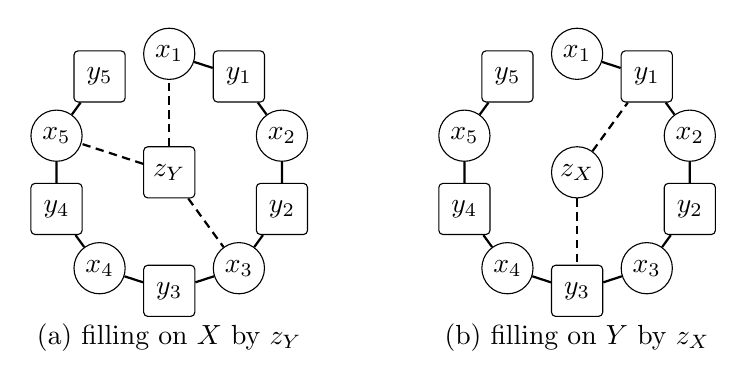
\begin{tikzpicture}[
				scale=0.7,
				xvertex/.style={circle,draw,minimum size=6.5mm,inner sep=1pt},
				yvertex/.style={rectangle,rounded corners=1.5pt,draw,
					minimum size=6.5mm,inner sep=1pt},
				cycleedge/.style={thick},
				fillingedge/.style={thick,densely dashed}
				]
				
				\begin{scope}[xshift=-3.7cm]
					\node[xvertex] (ax1) at (90:2.15) {$x_1$};
					\node[yvertex] (ay1) at (54:2.15) {$y_1$};
					\node[xvertex] (ax2) at (18:2.15) {$x_2$};
					\node[yvertex] (ay2) at (-18:2.15) {$y_2$};
					\node[xvertex] (ax3) at (-54:2.15) {$x_3$};
					\node[yvertex] (ay3) at (-90:2.15) {$y_3$};
					\node[xvertex] (ax4) at (-126:2.15) {$x_4$};
					\node[yvertex] (ay4) at (-162:2.15) {$y_4$};
					\node[xvertex] (ax5) at (162:2.15) {$x_5$};
					\node[yvertex] (ay5) at (126:2.15) {$y_5$};
					\node[yvertex] (azY) at (0,0) {$z_Y$};
					\draw[cycleedge]
					(ax1)--(ay1)--(ax2)--(ay2)--(ax3)--(ay3)--(ax4)--(ay4)--(ax5)--(ay5)--cycle;
					\draw[fillingedge] (azY)--(ax1);
					\draw[fillingedge] (azY)--(ax3);
					\draw[fillingedge] (azY)--(ax5);
					\node at (0,-3) {\textup{(a)} filling on \(X\) by \(z_Y\)};
				\end{scope}
				
				\begin{scope}[xshift=3.7cm]
					\node[xvertex] (bx1) at (90:2.15) {$x_1$};
					\node[yvertex] (by1) at (54:2.15) {$y_1$};
					\node[xvertex] (bx2) at (18:2.15) {$x_2$};
					\node[yvertex] (by2) at (-18:2.15) {$y_2$};
					\node[xvertex] (bx3) at (-54:2.15) {$x_3$};
					\node[yvertex] (by3) at (-90:2.15) {$y_3$};
					\node[xvertex] (bx4) at (-126:2.15) {$x_4$};
					\node[yvertex] (by4) at (-162:2.15) {$y_4$};
					\node[xvertex] (bx5) at (162:2.15) {$x_5$};
					\node[yvertex] (by5) at (126:2.15) {$y_5$};
					\node[xvertex] (bzX) at (0,0) {$z_X$};
					\draw[cycleedge]
					(bx1)--(by1)--(bx2)--(by2)--(bx3)--(by3)--(bx4)--(by4)--(bx5)--(by5)--cycle;
					\draw[fillingedge] (bzX)--(by1);
					\draw[fillingedge] (bzX)--(by3);
					\node at (0,-3){\textup{(b)} filling on \(Y\) by \(z_X\)};
				\end{scope}
			\end{tikzpicture}
			\caption{Solid edges form the induced cycle, and dashed edges show the two fillings}
			\label{fig:bifilled-cycle}
		\end{figure}
	\end{example}
	
	\begin{lemma}\label{lem:cycle-correspondence}
		Let \(G=(X\sqcup Y,E)\) be bipartite and \(q\ge4\).
		\begin{enumerate}[label=\textup{(\alph*)}]
			\item \(\CN(G)[X]\) contains an induced \(C_q\) if and only if \(G\)
			contains an induced \(C_{2q}\) with no filling on the \(X\) side.
			\item \(\CN(G)[Y]\) contains an induced \(C_q\) if and only if \(G\)
			contains an induced \(C_{2q}\) with no filling on the \(Y\) side.
		\end{enumerate}
	\end{lemma}
	
	\begin{proof}
		It is enough to prove \textup{(a)}, since interchanging \(X\) and \(Y\)
		gives \textup{(b)}.
		
		Suppose first that \(x_1,\ldots,x_q\) induce a cycle in \(\CN(G)[X]\),
		with indices read modulo \(q\). For each \(i\), select
		\[
		y_i\in N_G(x_i)\cap N_G(x_{i+1}).
		\]
		The selected vertices \(y_1,\ldots,y_q\) are distinct. If
		\(y_i=y_j\) for \(i\ne j\), then this vertex is adjacent to the endpoints of
		two different edges of the \(x\)-cycle. It would therefore create an edge of
		the common neighbor graph between two nonconsecutive vertices of the induced
		cycle. The same argument shows that, among the selected \(y\)-vertices,
		\(x_i\) is adjacent only to \(y_{i-1}\) and \(y_i\). Consequently,
		\[
		x_1y_1x_2y_2\cdots x_qy_qx_1
		\]
		is an induced \(C_{2q}\) in \(G\). This cycle has no filling on the \(X\)
		side, since a common neighbor of two nonconsecutive \(x_i\)'s would produce a
		chord of the
		induced cycle in \(\CN(G)[X]\).
		
		Conversely, suppose that
		\[
		x_1y_1x_2y_2\cdots x_qy_qx_1
		\]
		is an induced \(C_{2q}\) with no filling on the \(X\) side. Each consecutive pair
		\(x_i,x_{i+1}\) has the common neighbor \(y_i\), whereas no nonconsecutive
		pair of vertices in \(X\) on the cycle has a common neighbor. Hence
		\(x_1,\ldots,x_q\) induce a \(C_q\) in \(\CN(G)[X]\).
	\end{proof}
	
	\begin{proposition}\label{prop:cycle-filling}
		For a bipartite graph \(G=(X\sqcup Y,E)\), the graph \(\CN(G)\) is chordal
		if and only if every induced cycle of \(G\) of length at least eight is
		filled on both sides.
	\end{proposition}
	
	\begin{proof}
		By \eqref{eq:half-square-decomposition}, \(\CN(G)\) is chordal exactly when
		both half squares, \(\CN(G)[X]\) and \(\CN(G)[Y]\), are chordal.
		Lemma~\ref{lem:cycle-correspondence} shows that a hole \(C_q\), \(q\ge4\),
		in the half square on \(X\) corresponds to an induced \(C_{2q}\) in \(G\) with
		no filling on the \(X\) side. The symmetric statement holds for the half
		square on \(Y\). Thus neither half square contains a hole if and only if every
		induced cycle of
		\(G\) of length at least eight has a filling on \(X\) and a filling on
		\(Y\).
	\end{proof}
	
	Proposition~\ref{prop:cycle-filling} expresses the \(X\)-chordal and
	\(Y\)-chordal conditions in terms of half squares; see
	\cite[Theorems~6--7]{BrandstadtDraganChepoiVoloshin1998}. In that paper,
	the side label refers to the color class containing the bridge
	vertex. Here,
	a filling is labeled instead by the color class of the two cycle vertices that
	share that bridge vertex as a common neighbor. The following theorem therefore
	combines that classical bipartite hypertree characterization with
	Proposition~\ref{prop:background}.
	
	\begin{theorem}\label{thm:structural}
		For a nonempty finite simple graph \(G\), the following are equivalent:
		\begin{enumerate}[label=\textup{(\roman*)}]
			\item \(I_{\NN(G)}\) has a \(2\)-linear resolution over \(\Bbbk\);
			\item \(G\) is bipartite, its open neighborhoods form a Helly family, and
			every induced cycle of length at least eight is filled on both sides.
		\end{enumerate}
	\end{theorem}
	
	\begin{proof}
		Assume first that \textup{(i)} holds. By
		Proposition~\ref{prop:background}, the open neighborhoods of \(G\) form a
		Helly family and \(\CN(G)\) is chordal. We show that \(G\) is bipartite.
		
		First, \(G\) is triangle free. If \(G\) contained a triangle, it could be
		extended to a maximal clique \(Q\). Since \(|Q|\ge3\), every two vertices
		of \(Q\) have a third vertex of \(Q\) as a common neighbor. Hence \(Q\) is a
		clique of \(\CN(G)\). Lemma~\ref{lem:helly-flag} implies that \(Q\) is a face
		of \(\NN(G)\), so there exists \(w\in V(G)\) such that
		\[
		Q\subseteq N_G(w).
		\]
		Because \(G\) has no loops, \(w\notin Q\). Therefore \(Q\cup\{w\}\) is a
		clique of \(G\), contradicting the maximality of \(Q\). Hence \(G\) is triangle free.
		
		Suppose, toward a contradiction, that \(G\) is not bipartite. Let
		\[
		C=v_0v_1\cdots v_{m-1}v_0
		\]
		be a shortest odd cycle.
		The absence of triangles gives \(m\ge5\), and the minimality of \(m\)
		implies that \(C\) is induced. Since \(m\) is odd, multiplication by \(2\)
		permutes the residue classes modulo \(m\). The cyclic order
		\[
		v_0,v_2,v_4,\ldots,v_{2(m-1)},v_0,
		\]
		with indices taken modulo \(m\), therefore visits every vertex of \(C\).
		Consecutive vertices in this order are at distance two on \(C\), so they
		have a common neighbor on \(C\). They consequently form an \(m\)-cycle in
		\(\CN(G)\).
		
		We claim that this cycle is induced. Suppose that two vertices \(v_i\) and
		\(v_j\), nonconsecutive in this order, have a common neighbor
		\(w\). If \(w\in V(C)\), then the inducedness of \(C\) forces \(v_i\) and
		\(v_j\) to be the two neighbors of \(w\) on \(C\). They would then be
		consecutive in this order, a contradiction. Hence
		\(w\notin V(C)\).
		
		Exactly one of the two \(v_i\)--\(v_j\) arcs of \(C\) has odd length. Let
		\(\ell\) denote its length. If \(\ell=1\), then \(v_i,v_j,w\) form a triangle.
		If \(\ell=m-2\), then the complementary arc has length two, so \(v_i\) and
		\(v_j\) are consecutive in this order. Both cases are impossible,
		and therefore
		\[
		3\le\ell\le m-4.
		\]
		The odd arc, together with the edges \(v_iw\) and \(wv_j\), forms an odd
		cycle of length \(\ell+2<m\). This contradicts the choice of \(C\). Thus the
		cycle obtained from this order is induced and has length \(m\ge5\) in
		\(\CN(G)\),
		contrary to chordality. Hence \(G\) is bipartite.
		
		Proposition~\ref{prop:cycle-filling} now implies that every induced cycle of
		\(G\) of length at least eight is filled on both sides. Together with the
		Helly property of the open neighborhoods, this proves
		\textup{(ii)}.
		
		Conversely, assume \textup{(ii)}. By Proposition~\ref{prop:cycle-filling},
		the condition on induced cycles implies that \(\CN(G)\) is chordal. Since
		the open neighborhoods of \(G\) also form a Helly family,
		Proposition~\ref{prop:background} shows that \(I_{\NN(G)}\) has a \(2\)-linear resolution. Therefore
		\textup{(i)} holds.
	\end{proof}
	
	\begin{remark}
		A bipartite graph is \emph{chordal bipartite} if it has no induced cycle of
		length at least six. An induced \(C_6\) gives a triangle, rather than a
		hole, in each half square. The three vertices in either color class also
		determine pairwise intersecting open neighborhoods. If the open
		neighborhoods of \(G\) form a Helly family, each triple therefore
		has a common neighbor outside
		the cycle. Thus chordality of the half squares alone does not exclude an induced
		\(C_6\); the Helly condition in Theorem~\ref{thm:structural} is essential.
	\end{remark}
	
	\begin{corollary}\label{cor:chordal-bipartite}
		If \(G\) is a chordal bipartite graph without isolated vertices, then
		\(I_{\NN(G)}\) has a \(2\)-linear resolution.
	\end{corollary}
	
	\begin{proof}
		A chordal bipartite graph has no induced cycle of length at least six, so the
		condition on induced cycles in Theorem~\ref{thm:structural} is vacuous. It
		remains to prove that the open neighborhoods form a Helly family.
		
		Let \((N_G(x))_{x\in Q}\) be a pairwise intersecting indexed subfamily with at
		least two members. Since \(G\) is bipartite, all vertices of \(Q\) lie in the
		same color class. After interchanging the color classes if necessary, assume
		that \(Q\subseteq X\). If the total intersection were empty, there would be a subfamily indexed by
		\(Q'\subseteq Q\) that is minimal among those with empty intersection. Then
		\(|Q'|\ge3\), so there exist distinct \(x_1,x_2,x_3\in Q'\). By minimality, for each \(i\in\{1,2,3\}\) there
		exists
		\[
		y_i\in
		\bigcap_{x\in Q'\setminus\{x_i\}}N_G(x)
		\setminus N_G(x_i).
		\]
		The vertices \(y_1,y_2,y_3\) are distinct. Among the six selected vertices,
		\(y_i\) is adjacent to the two vertices \(x_j\) with \(j\ne i\), but not to
		\(x_i\). Hence
		\[
		x_1y_2x_3y_1x_2y_3x_1
		\]
		is an induced \(C_6\), contradicting chordal bipartiteness. Every pairwise
		intersecting subfamily with at least two members therefore has nonempty total
		intersection. Singleton subfamilies also intersect because \(G\) has no
		isolated vertices. Thus the open neighborhoods of \(G\) form a Helly family, and
		Theorem~\ref{thm:structural} gives the conclusion.
	\end{proof}
	
	\begin{remark}
		Corollary~\ref{cor:chordal-bipartite} applies, in particular, to every
		forest without isolated vertices and every chain graph without isolated
		vertices. It also recovers the \(2\)-linearity assertions for paths,
		stars, complete bipartite graphs, and \(2\times n\) grids obtained in
		\cite[Theorems~3.2, 3.4, 3.8, and 3.12]{Froberg2026}.
	\end{remark}
	

	A graph is a \emph{cactus graph} if any two cycles have at most one vertex in
	common. The structural criterion gives a particularly simple characterization
	within this class.

	\begin{theorem}\label{thm:cactus-characterization}
		Let \(G\) be a nonempty finite simple cactus graph. Then
		\(I_{\NN(G)}\) has a \(2\)-linear resolution if and only if \(G\) has no
		isolated vertices and every cycle of \(G\) has length four.
	\end{theorem}

	\begin{proof}
		Suppose first that \(I_{\NN(G)}\) has a \(2\)-linear resolution.
		Proposition~\ref{prop:background} shows that \(G\) has no isolated vertices,
		and Theorem~\ref{thm:structural} shows that \(G\) is bipartite and that its
		open neighborhoods form a Helly family.

		Every cycle of a cactus graph is induced, since a chord would produce two
		cycles with more than one common vertex. Moreover, no vertex outside a cycle
		can be adjacent to two vertices of that cycle, since the two additional edges
		and either suitable arc of the cycle would produce another cycle meeting the
		original one in at least two vertices.

		Because \(G\) is bipartite, every cycle has even length. Let \(C\) be a cycle
		of length at least eight. Theorem~\ref{thm:structural} requires a filling on
		each side of \(C\). Such a filling lies outside the induced cycle and is
		adjacent to two vertices of \(C\), contradicting the cactus property.

		A cycle of length six is also impossible. Let
		\[
		C=x_1y_1x_2y_2x_3y_3x_1.
		\]
		The neighborhoods \(N_G(x_1),N_G(x_2),N_G(x_3)\) intersect pairwise, since
		\[
		y_1\in N_G(x_1)\cap N_G(x_2),\qquad
		y_2\in N_G(x_2)\cap N_G(x_3),\qquad
		y_3\in N_G(x_3)\cap N_G(x_1).
		\]
		The Helly property gives a common neighbor of \(x_1,x_2,x_3\). This vertex
		lies outside \(C\) and is adjacent to at least two vertices of \(C\), again
		contradicting the cactus property. Hence every cycle of \(G\) has length four.

		Conversely, suppose that \(G\) has no isolated vertices and every cycle has
		length four. Then \(G\) is bipartite and has no induced cycle of length at
		least six. Thus \(G\) is chordal bipartite, and
		Corollary~\ref{cor:chordal-bipartite} gives the desired \(2\)-linear
		resolution.
	\end{proof}
	\begin{corollary}\label{cor:unique_cycle}
		The cycle graph \(C_4\) is the unique cycle graph \(C_n\) for which
		\(I_{\NN(C_n)}\) has a \(2\)-linear resolution.
	\end{corollary}
	
	\begin{proof}
		This is immediate from Theorem~\ref{thm:cactus-characterization}.
	\end{proof}
	
	\section{Constructions and closure properties}\label{sec:constructions}
	
	The first result gives a construction, followed by three closure properties.
	
	\begin{proposition}\label{prop:two-sided-cone}
		Let \(H=(X\sqcup Y,E(H))\) be a finite bipartite graph. Let \(x_0\) and
		\(y_0\) be
		two new vertices, and put
		\[
		\widehat X=X\cup\{x_0\},
		\qquad
		\widehat Y=Y\cup\{y_0\}.
		\]
		Define the bipartite graph \(\widehat H\) with color classes
		\(\widehat X\) and \(\widehat Y\) by
		\[
		E(\widehat H)
		=
		E(H)
		\cup
		\{x_0y:y\in Y\cup\{y_0\}\}
		\cup
		\{xy_0:x\in X\}.
		\]
		Then \(I_{\NN(\widehat H)}\) has a \(2\)-linear resolution over
		\(\Bbbk\).
	\end{proposition}
	
	\begin{proof}
		Every two vertices of \(\widehat X\) have the common neighbor \(y_0\), and
		every two vertices of \(\widehat Y\) have the common neighbor \(x_0\).
		Vertices in different color classes cannot have a common neighbor in a
		bipartite graph. Hence
		\[
		\CN(\widehat H)=K_{\widehat X}\sqcup K_{\widehat Y},
		\]
		which is chordal.
		
		It remains to prove that the open neighborhoods form a Helly family. Let
		\(Q\) be a
		clique of \(\CN(\widehat H)\). The displayed decomposition shows that either
		\(Q\subseteq\widehat X\) or \(Q\subseteq\widehat Y\). In the first case,
		\[
		Q\subseteq N_{\widehat H}(y_0),
		\]
		while in the second,
		\[
		Q\subseteq N_{\widehat H}(x_0).
		\]
		Thus every clique of \(\CN(\widehat H)\) is contained in an open
		neighborhood. Lemma~\ref{lem:helly-flag} implies that the open neighborhoods of
		\(\widehat H\) form a Helly family, and Proposition~\ref{prop:background} gives the
		result.
	\end{proof}
	
	For \(H=C_{2q}\) with \(q\ge3\), this class properly
	contains the chordal bipartite graphs without isolated vertices: the original
	cycle remains induced in \(\widehat H\), while the two new vertices provide
	fillings from the two color classes. Thus the construction produces admissible
	graphs with induced cycles of arbitrary even length.
	
	A \emph{false twin} of a vertex \(v\) is a nonadjacent vertex with the same open neighborhood as \(v\).
	
	\begin{proposition}
		\label{prop:closure-operations}
		The class of finite simple graphs \(G\) for which
		\(I_{\NN(G)}\) has a \(2\)-linear resolution is closed under the
		following operations:
		\begin{enumerate}[label=\textup{(\alph*)}]
			\item taking a nonempty finite disjoint union;
			\item adding a pendant vertex adjacent to an arbitrary vertex;
			\item adding a false twin of an arbitrary vertex.
		\end{enumerate}
	\end{proposition}
	
	\begin{proof}
		The proof uses Proposition~\ref{prop:background} and the clique formulation
		in Lemma~\ref{lem:helly-flag}.

		For \textup{(a)}, if \(G=G_1\sqcup\cdots\sqcup G_t\), then
		\[
		\CN(G)=\CN(G_1)\sqcup\cdots\sqcup\CN(G_t).
		\]
		This graph is chordal, and every clique lies in one component, where it is
		contained in an open neighborhood. Hence the open neighborhoods of \(G\)
		are Helly.

		For \textup{(b)}, let \(p\) be pendant at \(v\). The old induced subgraph
		of \(\CN(G')\) is \(\CN(G)\), and
		\[
		N_{\CN(G')}(p)=N_G(v),
		\]
		which is a clique because its vertices have the common neighbor \(v\).
		Thus \(p\) is simplicial and \(\CN(G')\) is chordal. A clique not
		containing \(p\) has an old common neighbor, while a clique containing
		\(p\) is contained in \(N_{G'}(v)\). Hence the new neighborhood family is
		Helly.

		For \textup{(c)}, let \(v'\) be a false twin of \(v\). Then
		\(\CN(G')[V(G)]=\CN(G)\), and \(v,v'\) are true twins in
		\(\CN(G')\). Adding a true twin to a chordal graph preserves chordality:
		an induced cycle containing only the new twin can be transferred to the old
		one, whereas a cycle containing both has a chord through their equal closed
		neighborhoods. Finally, if a clique \(Q\) contains \(v'\), replace \(v'\)
		by \(v\); an old common neighbor of the resulting clique is also a common
		neighbor of \(Q\), since \(N_{G'}(v')=N_G(v)\). Thus the open
		neighborhoods remain Helly in all three cases.
	\end{proof}
	
	The false twin hypothesis is essential: adding a true twin to an endpoint of
	\(K_2\) produces \(K_3\), which is excluded by
	Theorem~\ref{thm:structural}.
	
	\section{Multigraded and graded Betti numbers}\label{sec:betti}
	
	Throughout this section, assume that \(I_{\NN(G)}\) has a \(2\)-linear
	resolution, and set \(n=|V|\), \(H=\CN(G)\), and
	\(R=\Bbbk[\NN(G)]\). The common neighbor graph gives the multigraded
	Betti numbers, while subsets of the original graph with a common neighbor give
	the total Betti numbers.
	Proposition~\ref{prop:background} gives
	\[
	\NN(G)=\Cl(H)\qquad\text{and}\qquad H\text{ is chordal}.
	\]
	For \(W\subseteq V\), let \(c_H(W)\) denote the number of connected
	components of \(H[W]\), and write
	\[
	\beta_{i,W}(R)
	=
	\dim_{\Bbbk}\operatorname{Tor}_i(R,\Bbbk)_W
	\]
	for the squarefree multigraded Betti number indexed by \(W\).

	\begin{lemma}\label{lem:chordal-clique-contractible}
		If \(H\) is a nonempty connected chordal graph, then its clique complex
		\(\Cl(H)\) is contractible.
	\end{lemma}
	
	\begin{proof}
		We argue by induction on \(|V(H)|\). The result is immediate when \(H\) has
		one vertex. Assume that \(|V(H)|>1\). Since \(H\) is chordal, it has a simplicial vertex \(v\). Connectedness gives
		\(N_H(v)\ne\varnothing\).
		
		The graph \(H-v\) remains connected. If a path in \(H\) contains a
		segment \(x,v,y\), then \(x\) and \(y\) are adjacent because \(N_H(v)\) is a
		clique. Replacing the segment \(x,v,y\) by the edge \(xy\) removes \(v\)
		from the path. The graph \(H-v\) is also chordal, so the induction hypothesis
		implies that \(\Cl(H-v)\) is contractible.
		
		Every face of \(\Cl(H)\) containing \(v\) lies in the simplex on
		\(N_H[v]\). This simplex meets \(\Cl(H-v)\) in the nonempty simplex on
		\(N_H(v)\). Collapsing the simplex on \(N_H[v]\) onto this common face,
		relative to the intersection, collapses \(\Cl(H)\) onto \(\Cl(H-v)\).
		Since \(\Cl(H-v)\) is contractible, so is \(\Cl(H)\).
	\end{proof}


	\begin{theorem}\label{thm:all-betti}
		The multigraded Betti numbers of \(R=\Bbbk[\NN(G)]\) are
		\[
		\beta_{0,\varnothing}(R)=1,
		\qquad
		\beta_{0,W}(R)=0\quad(W\ne\varnothing),
		\]
		and, for \(i\ge1\),
		\begin{equation}\label{eq:multigraded}
			\beta_{i,W}(R)=
			\begin{cases}
				c_H(W)-1,& |W|=i+1,\\
				0,& |W|\ne i+1.
			\end{cases}
		\end{equation}
		Consequently, the only total Betti numbers in positive homological degrees are
		\begin{equation}\label{eq:component-total}
			\beta_{i,i+1}(R)=
			\sum_{\substack{W\subseteq V\\|W|=i+1}}
			\bigl(c_H(W)-1\bigr),\qquad 1\le i\le n-1.
		\end{equation}
		Equivalently, all Betti numbers of the ideal are
		\[
		\beta_{p,p+2}(I_{\NN(G)})
		=
		\sum_{\substack{W\subseteq V\\|W|=p+2}}
		\bigl(c_H(W)-1\bigr),\qquad 0\le p\le n-2,
		\]
		and \(\beta_{p,j}(I_{\NN(G)})=0\) for \(j\ne p+2\).
	\end{theorem}

	\begin{proof}
		Let \(W\subseteq V\). Since \(H\) is chordal, the induced subgraph \(H[W]\)
		is chordal as well. By Lemma~\ref{lem:chordal-clique-contractible}, the clique
		complex of each connected component of \(H[W]\) is contractible. Therefore,
		for \(W\ne\varnothing\), the complex \(\Cl(H[W])\) is a disjoint union of
		\(c_H(W)\) contractible complexes, and its only nonzero reduced homology is
		\[
		\dim_{\Bbbk}\widetilde H_0(\Cl(H[W]);\Bbbk)=c_H(W)-1.
		\]
		
		Hochster's formula \cite{Hochster1977} now gives, for \(i\ge1\),
		\[
		\beta_{i,W}(R)
		=
		\dim_{\Bbbk}\widetilde H_{|W|-i-1}
		\bigl(\Cl(H[W]);\Bbbk\bigr)
		=
		\begin{cases}
			c_H(W)-1,&|W|=i+1,\\
			0,&|W|\ne i+1.
		\end{cases}
		\]
		For \(W=\varnothing\), the standard convention gives
		\(\beta_{0,\varnothing}(R)=1\), while all other multigraded Betti numbers in
		homological degree zero vanish. This agrees with the formula of Engstr\"om and
		Stamps \cite{EngstromStamps2013} for clique complexes of chordal
		graphs.
		
		Summing over all subsets \(W\) with \(|W|=i+1\) gives
		\eqref{eq:component-total}. Finally, the exact sequence
		\[
		0\longrightarrow I_{\NN(G)}\longrightarrow S\longrightarrow R
		\longrightarrow0
		\]
		shifts the positive homological degrees by one. Hence
		\[
		\beta_{p,p+2}(I_{\NN(G)})=\beta_{p+1,p+2}(R),
		\]
		which yields the asserted Betti numbers of the ideal.
	\end{proof}
	

\begin{thebibliography}{99}
\bibitem[BrandstadtDraganChepoiVoloshin1998]{BrandstadtDraganChepoiVoloshin1998} A. Brandst\"adt, F. Dragan, V. Chepoi and V. Voloshin, \emph{Dually chordal graphs}, SIAM J. Discrete Math. \textbf{11} (1998), no.~3, 437--455. \href{https://doi.org/10.1137/S0895480193253415}{doi:\nolinkurl{10.1137/S0895480193253415}}.
\bibitem[EngstromStamps2013]{EngstromStamps2013} A. Engstr\"om and M. T. Stamps, \emph{Betti diagrams from graphs}, Algebr. Number Theory \textbf{7} (2013), no.~7, 1725--1742. \href{https://doi.org/10.2140/ant.2013.7.1725}{doi:\nolinkurl{10.2140/ant.2013.7.1725}}.
\bibitem[Froberg1990]{Froberg1990} R. Fr\"oberg, \emph{On Stanley--Reisner rings}, Banach Center Publ. \textbf{26}, Part~2 (1990), 57--70. \href{https://doi.org/10.4064/-26-2-57-70}{doi:\nolinkurl{10.4064/-26-2-57-70}}.
\bibitem[Froberg2026]{Froberg2026} R. Fr\"oberg, \emph{Stanley--Reisner rings of neighborhood complexes and linear resolutions}, J. Algebraic Combin. \textbf{63} (2026), article~56. \href{https://doi.org/10.1007/s10801-026-01530-x}{doi:\nolinkurl{10.1007/s10801-026-01530-x}}.
\bibitem[Hochster1977]{Hochster1977} M. Hochster, \emph{Cohen--Macaulay rings, combinatorics, and simplicial complexes}, in \emph{Ring Theory II (Proc. Second Oklahoma Ring Theory Conference, Norman, 1975)}, Lecture Notes in Pure and Applied Mathematics, vol.~26, Marcel Dekker, New York, 1977, 171--223.
\bibitem[LeLe2019]{LeLe2019} H.-O. Le and V. B. Le, \emph{Hardness and structural results for half-squares of restricted tree convex bipartite graphs}, Algorithmica \textbf{81} (2019), 4258--4274. \href{https://doi.org/10.1007/s00453-018-0440-7}{doi:\nolinkurl{10.1007/s00453-018-0440-7}}.
\end{thebibliography}
\end{document}
